
\section{Einordnung und weitere Visualisierung der Daten}
Im folgenden wird die Korrelation der Corona-Fälle der einzelnen deutschen Landkreise untersucht. Um dieses Verfahren besser zu verstehen und ein grobes Gefühl für den Datensatz zu bekommen, werden die einzelnen Werte gesondert an.

\subsection{Die deutschen Landkreise und Ihre Bevölkerungsdichte}
Zuallererst folgen die genutzten Daten, welche nichts mit Corona zutun haben: Die Landkreise und ihre Bevölkerungsdichte. Die Bevölkerungsdichte wird aus der Bevölkerungszahl und der Fläche des Landkreises berechnet, welche von der API bereitgestellt werden \todo{adäquate Verlinkung auf API}.

In Abbildung \autoref{fig:distribution_pop_density_counties} sind die Bevölkerungsdichten der einzelnen Landkreise dargestellt. Auf der linken Seite befindet sich die Verteilung und auf der rechten Seite die räumliche Anordnung.
Die Bezirke Berlins sind einzeln gelistet, daher entsprechen die sechs höchsten Bevölkerungsdichten den Berliner Bezirken  Friedrichshain-Kreuzberg, Mitte, Neukölln, Tempelhof-Schöneberg, Lichtenberg, Charlottenburg-Wilmersdorf, obwohl die Bevölkerungsdichte des gesamten Berliner Stadtkreises niedriger ist als die Bevölkerungsdichte Münchens (in dieser Auflistung Platz 7, ohne Berliner Bezirke Platz 1).

\begin{figure}[H]
    \centering
    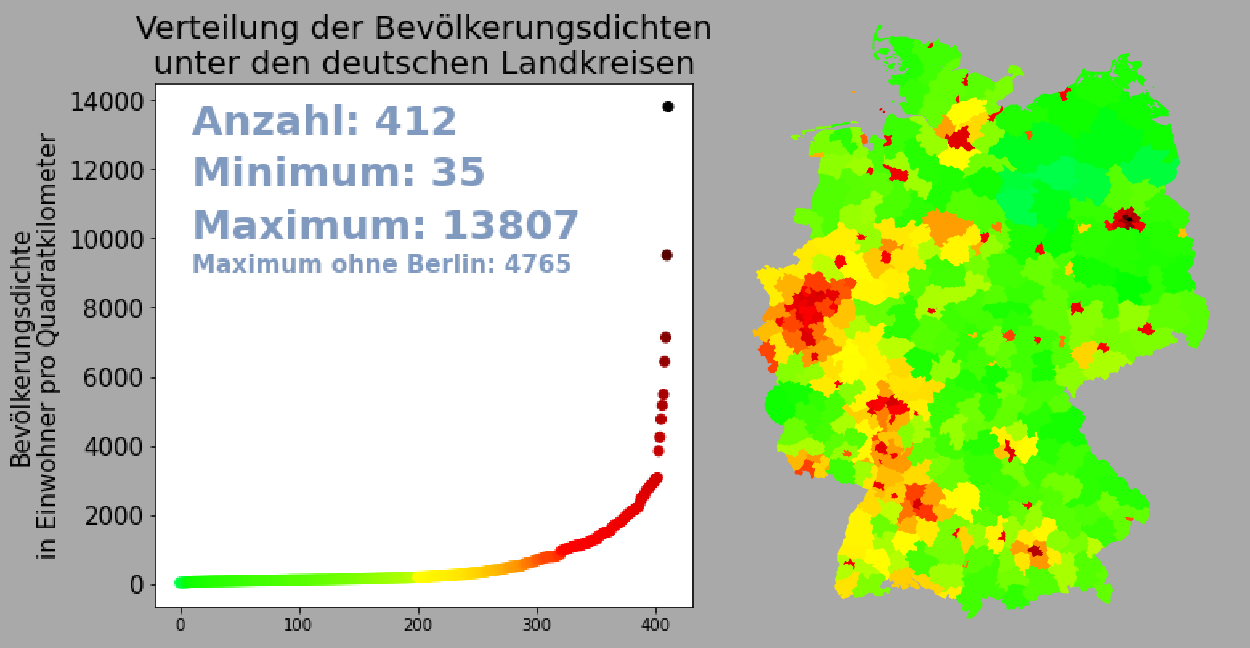
\includegraphics[width = 0.95\textwidth]{figures/Durchführung/population_density_counties_Distribution_and_map.png}
    \caption{Verteilung der Bevölkerungsdichten unter den deutschen Landkreisen.}
    \label{fig:distribution_pop_density_counties}
\end{figure}

\todo{klarstellen, das die Landkreise nicht den Landkreisen entsprechen (Berlin ist aufgeteilt) Aus Wikipedia "Landkreis": In Deutschland gibt es 294 Landkreise. Zusammen mit den 106 kreisfreien Städten bilden sie die insgesamt 400 Gebietskörperschaften auf Kreisebene. Wir haben 412.}
In Abbildung 


Teilt man die Landkreise nach den ersten beiden Kennzahlen des Landkreises, die des Bundeslandes und die des aktuellen (teils auch vergangenen) Regierungsbezirks, ein, ergibt sich für die Bevölkerungsdichte das in \autoref{fig:distribution_pop_density_districts} dargestellte Bild.

Nicht alle Bundesländer wurden in Regierungsbezirke unterteilt, in diesem Fall wird die Bevölkerungsdichte des Landkreises gewählt. Im folgenden wird dennoch von \glqq{}den Regierungsbezirken\grqq{} gesprochen. Zudem sind die Stadtstaaten Bremen und Hamburg zum Regierungsbezirk Lüneburg hinzugefügt und der Stadtstaat Berlin zum Bundesland Brandenburg hinzugefügt.

\begin{figure}[H]
    \centering
    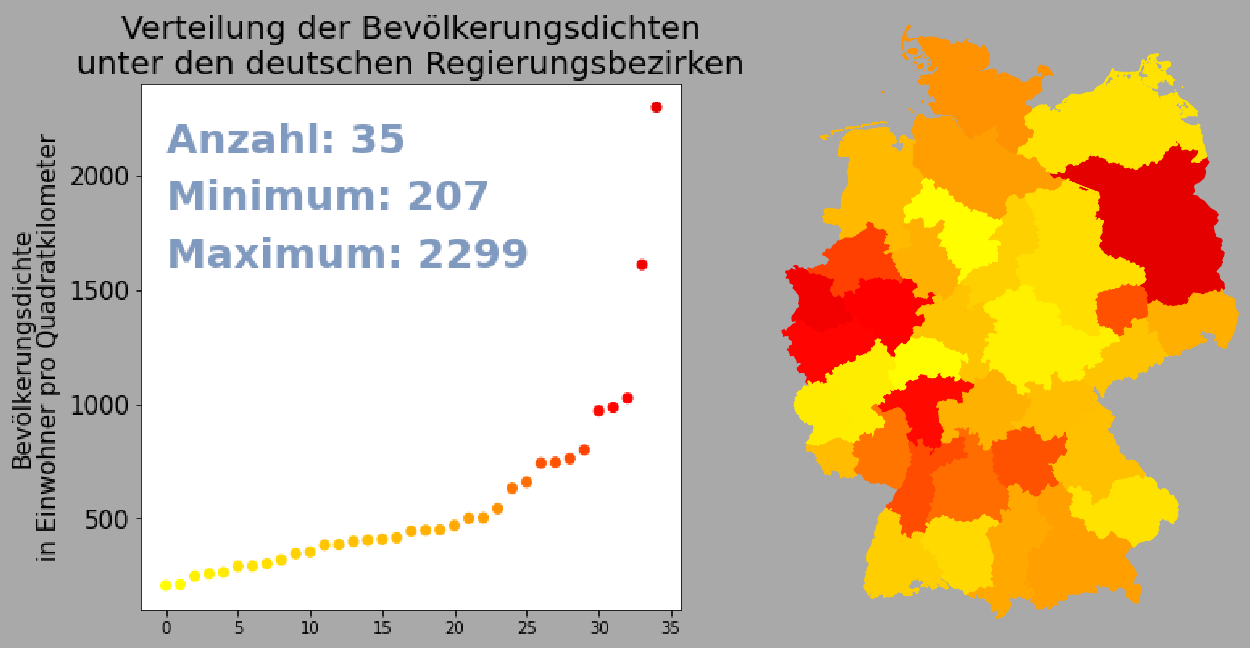
\includegraphics[width = 0.95\textwidth]{figures/Durchführung/population_density_districts_Distribution_and_map.png}
    \caption{Verteilung der Bevölkerungsdichten unter den deutschen Regierungsbezirken. Die Skalierung entspricht der Farbgebung in \autoref{fig:distribution_pop_density_counties}.}
    \label{fig:distribution_pop_density_districts}
\end{figure}

Klar zu erkennen sind die Stadtkreise in Abbildung \ref{fig:distribution_pop_density_counties}: Sie weisen eine hohe Bevölkerungsdichte auf und sind in der Regel von weniger stark bevölkerten Landkreisen umgeben.

Die Städte in Tabelle \ref{tab:landkreise_um_städte} von einem Landkreis umgeben, an Ihnen lässt sich besonders gut testen, ob sich in den Korrelationswahrscheinlichkeiten zwischen einer Stadt und ihrem Umland eine zeitliche Verschiebung feststellen lässt.
\begin{table}[H]
    \centering
    \begin{tabular}{c}
Kassel 6633\\
Trier-Saarburg 7235\\
Südliche Weinstraße 7337\\
Südwestpfalz 7340\\
Heilbronn 8125\\
Rastatt 8216\\
Rosenheim 9187\\
Landshut 9274\\
Straubing-Bogen 9278\\
Amberg-Sulzbach 9371\\
Beustadt a.d. Waldnaab 9374\\
Regensburg 9375\\
Bamberg 9471\\
Bayreuth 9472\\
Coburg 9473\\
Hof 9475\\
Ansbach 9571\\
Schweinfurt 9678\\
Würzburg 9679\\
Ostallgäu 9777\\
Oberallgäu 9780\\
Potsdam-Mittelmark 12069\\
Spree-Neiße 12071\\
Saalekreis 15088\\
Weimarer Land 16071\\
\todo{fill table}
    \end{tabular}
    \caption{Landkreise mit Name und Gemeindeschlüssel, die eine Stadt komplett umgeben.}
    \label{tab:landkreise_um_städte}
\end{table}
Als erstes Beispiel zu Demonstrationszwecken ausführlich gezeigt.

